% SPDX-License-Identifier: CC-BY-4.0
% Copyright (C) 2026 Fabian Januszewski, Abhijit and the Langlandscape team
% S03-T1: Gamma_U\T_q collapses onto the 2-vertex DR graph; kernel = Ribet sequence.  Case B_11, q=2 (D=11).
% math: mathematics/chapters/s03/3-ribet.tex  lem:s03-bip, thm:s03-ribet(a);  mathematics/chapters/s03/1-graphs.tex  def:s03-DR, def:s03-graph, prop:s03-phi
% data: code/results/s03/T2.json (case B11_q2: s0, s1, w_edges, collapse_two_vertex_weights, phi_collapsed_order, rk_H1, T_q_eigenvalues, cusp_det_q1sq_minus_lam_sq, acceptance_note)
\begin{frame}{Collapse: $\Gamma_U\backslash\mathcal T_q\ \to$ DR graph; the kernel is Ribet's sequence}
  \centering
  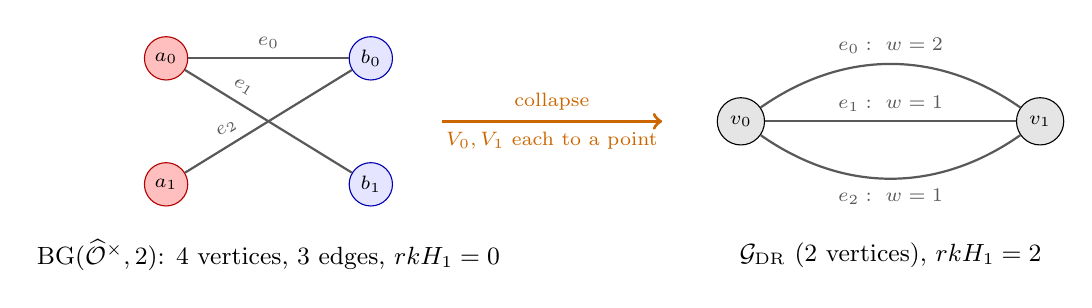
\begin{tikzpicture}[every node/.style={font=\scriptsize},
      va/.style={circle,draw=red!70!black,fill=red!25,inner sep=1pt,minimum size=5.5mm},
      vb/.style={circle,draw=blue!70!black,fill=blue!10,inner sep=1pt,minimum size=5.5mm},
      vc/.style={circle,draw=black,fill=gray!20,inner sep=1pt,minimum size=6mm},
      ed/.style={thick,gray!70!black}]
    % BG(Ohat^x,2): s_0 = (0,0,1), s_1 = (0,1,0) on the 3 edges
    \node[va] (a0) at (0,1.0) {$a_0$};
    \node[va] (a1) at (0,-0.6) {$a_1$};
    \node[vb] (b0) at (2.6,1.0) {$b_0$};
    \node[vb] (b1) at (2.6,-0.6) {$b_1$};
    \draw[ed] (a0) -- node[above] {$e_0$} (b0);
    \draw[ed] (a0) -- node[pos=0.3,above,sloped] {$e_1$} (b1);
    \draw[ed] (a1) -- node[pos=0.3,above,sloped] {$e_2$} (b0);
    \node[font=\small] at (1.3,-1.5) {$\mathrm{BG}(\widehat{\mathcal O}^\times,2)$: $4$ vertices, $3$ edges, $\operatorname{rk}H_1=0$};
    % collapse arrow
    \draw[->,very thick,orange!80!black] (3.5,0.2) -- node[above] {collapse} node[below] {$V_0,V_1$ each to a point} (6.3,0.2);
    % collapsed graph
    \node[vc] (u) at (7.3,0.2) {$v_0$};
    \node[vc] (v) at (11.1,0.2) {$v_1$};
    \draw[ed] (u) to[bend left=35]  node[above] {$e_0:\ w=2$} (v);
    \draw[ed] (u) -- node[above] {$e_1:\ w=1$} (v);
    \draw[ed] (u) to[bend right=35] node[below] {$e_2:\ w=1$} (v);
    \node[font=\small] at (9.2,-1.5) {$\mathcal G_{\mathrm{DR}}$ (2 vertices), $\operatorname{rk}H_1=2$};
  \end{tikzpicture}

  \vspace{-1mm}
  \begin{itemize}\small
    \item \textbf{Ribet sequence} (thm.\ s03-ribet(a), lem.\ s03-bip): with $E=X_{U'}$, $X=X_U$, $\alpha=(-s_{0*},s_{1*})$,
      \[0\to H_1(\mathrm{BG})\to \mathbb Z[E]^0\xrightarrow{\ \alpha\ }\big(\mathbb Z[X]^0\big)^2\to 0,
        \qquad \text{here } 0\to 0\to\mathbb Z^2\xrightarrow{\ \sim\ }\mathbb Z^2\to 0 .\]
      The collapse keeps all edges, so $H_1(\mathcal G_{\mathrm{DR}})=\mathbb Z[E]^0$ (prop.\ s03-phi).
    \item $|\Phi^{\mathrm{comb}}|=\big(\prod_e w_e\big)\sum_e \tfrac1{w_e}=2\cdot\big(\tfrac12+1+1\big)=5$.
    \item $T_2$ on the cuspidal eigenspace: $\lambda=-2$, and $(q+1)^2-\lambda^2=9-4=5$ (computed).
  \end{itemize}
  \vfill
  {\tiny Sources: \texttt{code/results/s03/T2.json} (\texttt{B11\_q2}: \texttt{s0}, \texttt{s1}, \texttt{w\_edges}, \texttt{phi\_collapsed\_order}, \texttt{cusp\_det\_q1sq\_minus\_lam\_sq}); thm.\ s03-ribet, lem.\ s03-bip, prop.\ s03-phi; status: proved / computed.}
\end{frame}
